\documentclass[a4paper,10pt,twoside,final,spanish]{article}

% Preámbulo - Parte A

\usepackage[utf8]{inputenc} % Soporte para los acentos
\usepackage[T1]{fontenc}

\usepackage[spanish]{babel} % Capítulos, seciones, etc. en español

\usepackage[margin=2cm]{geometry} % Diseño del documento

\usepackage{multicol} % Escribir doble columna

\usepackage{xcolor} % Usar colores
\usepackage{pstricks}

\usepackage{enumerate} % Cambiar etiquetas de numeración
\usepackage[shortlabels]{enumitem} % Manejo adicional de etiquetas de numeración

\usepackage{graphicx} % Manejo de gráficos y figuras

\usepackage{makeidx} % Índice alfabético

% Paquetes adicionales de símbolos matemáticos
\usepackage{amsmath,amssymb,amsfonts,latexsym} 

% \usepackage{pslatex} % Fuente Times
% \usepackage{mathpazo} % Fuente Palatino
% \usepackage{mathptmx} % Fuente Times
% \usepackage{bookman} % Fuente Bookman
\usepackage{newcent} % Fuente New Century Schoolbook
% \usepackage{helvet} % Fuente Helvetica
% \usepackage{palatino} % Fuente Palatino
% \usepackage{pxfonts} % Fuente 
% \usepackage{txfonts} % Fuente
% \usepackage{concrete} % Fuente
% \usepackage{cmbright} % Fuente
% \usepackage{fourier} % Fuente

\usepackage{booktabs} % Opciones adicionales para el entorno tabular
\usepackage{longtable} % Para tablas de más de una página

\usepackage{tikz} % Creación de gráficos

\usepackage{hyperref}

\usepackage{gensymb} % Grados Celcius

\usepackage{booktabs} % Opciones adicionales para el entorno tabular
\usepackage{longtable} % Para tablas de más de una página

\usepackage{tikz,tkz-tab} % Creación de gráficos
	\usetikzlibrary{matrix,arrows,positioning,shadows,shadings,
					backgrounds,calc,shapes,tikzmark}
\usepackage{tcolorbox,empheq} % Creación de cajas
	\tcbuselibrary{skins,breakable,listings,theorems}
	
%	\tcbset{opteqC/.style={skin=beamer,colback=red!5!white}}

\usepackage{textcomp}

\usepackage[makeroom]{cancel} %Para tachar expresiones matemáticas
\newcommand\Ccancel[2][black]{\renewcommand\CancelColor{\color{#1}}\cancel{#2}}

\usepackage{titlesec}

\titleformat{\section} % command
			[display] % shape
			{\usefont{T1}{phv}{b}{n}\LARGE} % format
			{} % label
			{1pt} % sep
			{\thesection.\hspace{0.5em}} % before code
			
\titleformat{\subsection} % command
			[display] % shape
			{\usefont{T1}{phv}{b}{n}\Large} % format
			{} % label
			{1pt} % sep
			{\thesubsection.\hspace{0.5em}} % before code
			
\titleformat{\subsubsection} % command
			[display] % shape
			{\usefont{T1}{phv}{b}{n}\large} % format, fuentes: lmss,pag,phv
			{} % label
			{1pt} % sep
			{\thesubsubsection.\hspace{0.5em}} % before code		

\titleformat{name=\section,numberless}
			[display]
			{\usefont{T1}{phv}{b}{n}\LARGE}
			{}
  			{1pt}
  			{}
			\titlespacing*{\section}{0pt}{1pt}{1pt}

\usepackage{soul} % para tachar texto
\pagestyle{headings}
% Para encerrar expresiones con círculos
\usepackage{mathtools}% superior to amsmath
\usepackage{siunitx} % para escribir grados minutos segundos
\usepackage{tikz}
\makeatletter
\newcommand\mathcircled[1]{%
  \mathpalette\@mathcircled{#1}%
}
\newcommand\@mathcircled[2]{%
  \tikz[baseline=(math.base)] \node[draw,circle,inner sep=1pt] (math) {$\m@th#1#2$};%
}
\makeatother
%---
\usepackage{fancyhdr} %Para usar encabezados y pies personalizados
	\pagestyle{fancy}
	\fancyhf{}
	\fancyhead[LE,RO]{Mecánica del Continuo}
	\fancyhead[RE,LO]{Ecuaciones de Campo y Condiciones de Contorno}
	\fancyfoot[LE,RO]{\thepage}
	\fancyfoot[RE,LO]{Darién Julián Ramírez}	
	\renewcommand{\footrulewidth}{1pt}
%---
\usepackage{listings} %Para escribir códigos
\lstset{language=XML,
	basicstyle=\footnotesize,
	numbers=left,
 	stepnumber=1,
	numbersep=8pt,
	showspaces=false,               % show spaces adding particular underscores
  	showstringspaces=false,         % underline spaces within strings
  	frame=lines,                   % adds a frame around the code
	tabsize=4,                      
  	captionpos=b,                   % sets the caption-position to bottom
  	breaklines=true,                % sets automatic line breaking
}
%---

% Preámbulo - Parte B

\title{\Huge\usefont{T1}{lmss}{b}{n} Mecánica del Continuo \\
			 Trabajo Práctico Nº9  \\
			 Ecuaciones de Campo \\ y \\ Condiciones de Contorno}
\author{Darién Julián Ramírez}
\date{}

% Cuerpo del documento

\begin{document}

\maketitle % Mostrar título

\section*{Ejercicio 1}

Sea $V$ el volumen encerrado por la superficie $S$ cuya normal saliente unitaria es $\nu$; y sea $x$ el vector posición en un punto en $V$. Usando el \textit{teorema de Gauss} y notación indicial mostrar que: \\

\begin{quote}
\begin{tcolorbox}[colback=gray!10!white,colframe=black!0!white]

\textit{Teorema de Gauss (transforma integrales de superficie en integrales de volumen):}

\begin{align*}
\int_{V}\frac{\partial A}{\partial x_{i}}dV=\int_{S}A\nu_{i}dS
\end{align*}

\end{tcolorbox}
\end{quote}

\begin{enumerate}[a.]
\item \begin{align*}
\int_{S}x_{i}\nu_{j}dS &= V\delta_{ij}
\end{align*}

\begin{quote}
\begin{tcolorbox}[colback=gray!10!white,colframe=black!0!white]

\begin{align*}
\int_{S}x_{i}\nu_{j}dS &= \int_{V}\frac{\partial x_{i}}{\partial x_{j}}dV 
& \frac{\partial x_{i}}{\partial x_{j}} &= \delta_{ij} \\
&= \int_{V}\delta_{ij}\,dV \\ 
&= \delta_{ij}\int_{V}dV \\
&= \delta_{ij}V \\
\end{align*}

\end{tcolorbox}
\end{quote}

\item \begin{align*}
\int_{S}\nu\times(\mathbf{a}\times\mathbf{x})dS &= 2V\mathbf{a};
& \mathbf{a} &= \textit{vector arbitrario constante independiente de x}
\end{align*}

\begin{quote}
\begin{tcolorbox}[colback=gray!10!white,colframe=black!0!white]

\begin{align*}
\int_{S}\nu\times(\mathbf{a}\times\mathbf{x})\,dS
&= \int_{S}\varepsilon_{ijk}\nu_{j}(\mathbf{a}\times\mathbf{x})_{k}\,dS \\
&= \int_{S}\varepsilon_{ijk}\nu_{j}\varepsilon_{kem}a_{e}x_{m}\,dS \\
&= \int_{S}\varepsilon_{ijk}\varepsilon_{kem}\nu_{j}a_{e}x_{m}\,dS \\
&= \int_{S}\varepsilon_{kij}\varepsilon_{kem}\nu_{j}a_{e}x_{m}\,dS \\
&= \int_{S}(\delta_{ie}\delta_{jm}-\delta_{im}\delta_{je})\nu_{j}a_{e}x_{m}\,dS \\
&= \int_{S}(\delta_{ie}\delta_{jm}\nu_{j}a_{e}x_{m}
-\delta_{im}\delta_{je}\nu_{j}a_{e}x_{m})\,dS \\
&= \int_{S}(\delta_{jm}\nu_{j}a_{i}x_{m}-\delta_{je}\nu_{j}a_{e}x_{i})\,dS \\
&= \int_{S}(\nu_{j}a_{i}x_{j}-\nu_{j}a_{j}x_{i})\,dS \\
&= \int_{S}\nu_{j}a_{i}x_{j}\,dS-\int_{S}\nu_{j}a_{j}x_{i}\,dS \\
&= \int_{S}a_{i}x_{j}\nu_{j}\,dS-\int_{S}a_{j}x_{i}\nu_{j}\,dS \\
&= \int_{V}{\red \frac{\partial}{\partial x_{j}}(a_{i}x_{j})}\,dV
-\int_{V}{\blue \frac{\partial}{\partial x_{j}}(a_{j}x_{i})}\,dV \\ \\
{\red \frac{\partial}{\partial x_{j}}(a_{i}x_{j})}
&= {\red a_{i}\frac{\partial x_{j}}{\partial x_{j}}=a_{i}\delta_{jj}=3a_{i}} \\ \\
{\blue \frac{\partial}{\partial x_{j}}(a_{j}x_{i})}
&= {\blue a_{j}\frac{\partial x_{i}}{\partial x_{j}}=a_{j}\delta_{ij}=a_{i}} \\ \\
&= \int_{V}{\red 3a_{i}}\,dV-\int_{V}{\blue a_{i}}\,dV \\
&= 3a_{i}\int_{V}\,dV-a_{i}\int_{V}\,dV \\
&= 3a_{i}V-a_{i}V \\
&= 2a_{i}V \\
&= 2\mathbf{a}V
\end{align*}

\end{tcolorbox}
\end{quote}

\item \begin{align*}
\int_{S}\lambda\mathbf{w}\nu\,dS &= \int_{V}\mathbf{w}\cdot\nabla\lambda dV;
& \mathbf{w} &= rot(\mathbf{v}) \\
&& \mathbf{v} &= \mathbf{v}(\mathbf{x})= \textit{ función vectorial arbitraria} \\
&& \lambda &= \lambda(\mathbf{x})= \textit{ función escalar arbitraria}
\end{align*}

\begin{quote}
\begin{tcolorbox}[colback=gray!10!white,colframe=black!0!white]

\begin{align*}
\int_{S}\lambda\mathbf{w}\nu\,dS &= \int_{S}\lambda w_{i}\nu_{i}\,dS \\
&= \int_{S}\lambda (\nabla\times\mathbf{v})_{i}\nu_{i}\,dS \\
&= \int_{S}\lambda\varepsilon_{ijk}\frac{\partial v_{k}}{\partial x_{j}}\nu_{i}\,dS \\
&= \int_{V}\frac{\partial}{\partial x_{i}}
\left(\lambda\varepsilon_{ijk}\frac{\partial v_{k}}{\partial x_{j}}\right)\,dV \\
&= \int_{V}\frac{\partial}{\partial x_{i}}
\left(\varepsilon_{ijk}\lambda\frac{\partial v_{k}}{\partial x_{j}}\right)\,dV \\
&= \int_{V}\varepsilon_{ijk}
\left(\frac{\partial\lambda}{\partial x_{i}}\frac{\partial v_{k}}{\partial {x_{j}}}
+\lambda\frac{\partial v_{k}^{2}}{\partial x_{i}\partial x_{j}}\right)\,dV \\
&= \int_{V}
\left(\varepsilon_{ijk}\frac{\partial\lambda}{\partial x_{i}}\frac{\partial v_{k}}{\partial x_{j}}
+{\red \varepsilon_{ijk}\lambda\frac{\partial v_{k}^{2}}{\partial x_{i}\partial x_{j}}}\right)\,dV \\ \\
{\red \varepsilon_{ijk}\lambda\frac{\partial v_{k}^{2}}{\partial x_{i}\partial x_{j}}}
&= {\red \varepsilon_{ijk}\lambda\partial v_{k,ij}} \\
&= {\red \varepsilon_{ijk}\lambda
\left(\frac{1}{2}\partial v_{k,ij}+\frac{1}{2}\partial v_{k,ij}\right)} \\
&= {\red \frac{1}{2}\lambda
\left(\varepsilon_{ijk}\partial v_{k,ij}+\varepsilon_{ijk}\partial v_{k,ij}\right)} \\
&= {\red \frac{1}{2}\lambda
\left(\varepsilon_{ijk}\partial v_{k,ij}+\varepsilon_{jik}\partial v_{k,ji}\right)} \\
&= {\red \frac{1}{2}\lambda
\left(\partial v_{k,ij}-\partial v_{k,ji}\right)}
& {\red \partial v_{k,ij}} &= {\red \partial v_{k,ji}} \\
&= {\red \frac{1}{2}\lambda\cdot 0} \\
&= {\red 0} \\ \\
&= \int_{V}\varepsilon_{ijk}
\frac{\partial\lambda}{\partial x_{i}}\frac{\partial v_{k}}{\partial x_{j}}\,dV \\
&= \int_{V}\varepsilon_{ijk}
\frac{\partial v_{k}}{\partial x_{j}}\frac{\partial\lambda}{\partial x_{i}}\,dV \\
&= \int_{V}(\nabla\times\mathbf{v})\nabla\lambda\,dV \\
&= \int_{V}\mathbf{w}\cdot\nabla\lambda\,dV \\
\end{align*}

\end{tcolorbox}
\end{quote}

\end{enumerate}

\section*{Ejercicio 2}

Sea el movimiento de un cierto medio continuo descrito por las ecuaciones:

\begin{align*}
x_{1} &= a_{1}e^{-t}
& x_{2} &= a_{2}e^{t}
& x_{3} &= a_{3}+a_{2}(e^{-t}-1) 
\end{align*}

El campo de temperaturas en dicho medio está dado por:

\begin{align*}
T(x_{1},x_{2},x_{3},t) &= e^{-t}(x_{1}-2x_{2}+3x_{3})
\end{align*}

Calcule la derivada material de la temperatura en ese medio.

\dotfill

\begin{quote}
\textit{Derivada material:}

\begin{align*}
\frac{DA}{Dt}=\frac{\partial A}{\partial t}+\mathbf{\nu}\cdot\nabla A
=\frac{\partial A}{\partial t}+\nu_{i}\cdot\frac{\partial A}{\partial x_{i}}
=\frac{\partial A}{\partial t}+\left(
\nu_{1}\frac{\partial A}{\partial x_{1}}
+\nu_{2}\frac{\partial A}{\partial x_{2}}
+\nu_{3}\frac{\partial A}{\partial x_{3}}
\right)
\end{align*}

\begin{align*}
\frac{\partial T}{\partial t} &= -e^{-t}(x_{1}-2x_{2}+3x_{3}) 
\end{align*}

\begin{align*}
a_{1} &= x_{1}e^{t}
& \nu_{i} &= \frac{\partial x_{i}}{\partial t}
& \frac{\partial x_{1}}{\partial t} &= -a_{1}e^{-t}=-x_{1} \\
a_{2} &= x_{2}e^{-t}
&&& \frac{\partial x_{2}}{\partial t} &= a_{2}e^{t}=x_{2} \\
&&&& \frac{\partial x_{3}}{\partial t} &= -a_{2}e^{-t}=-x_{2}e^{-2t}
\end{align*}

\begin{align*}
\frac{\partial T}{\partial x_{1}} &= e^{-t} \\
\frac{\partial T}{\partial x_{2}} &= -2e^{-t} \\
\frac{\partial T}{\partial x_{3}} &= 3e^{-t}
\end{align*}

\begin{align*}
\frac{DT}{Dt} &= \frac{\partial T}{\partial t}+\nu_{i}\cdot\frac{\partial T}{\partial x_{i}}\\
&= -e^{-t}(x_{1}-2x_{2}+3x_{3})
+\left(-x_{1}\cdot e^{-t}+x_{2}\cdot(-2e^{-t})+(-x_{2}e^{-2t})\cdot3e^{-t}\right) \\
&= -x_{1}e^{-t}+2x_{2}e^{-t}-3x_{3}e^{-t}-x_{1}e^{-t}-2x_{2}e^{-t}-3x_{2}e^{-2t}e^{-t} \\
&= -2x_{1}e^{-t}-3x_{3}e^{-t}-3x_{2}e^{-2t}e^{-t} \\
&= (-2x_{1}-3x_{3}-3x_{2}e^{-2t})e^{-t} \\
\end{align*}

\end{quote}

\section*{Ejercicio 3}

Dos componentes del campo de velocidad de un fluido son conocidas para una región $-2\leq x,y,z\leq 2$:

\begin{align*}
u &= (1-y^{2})(a+bx+cx^{2}) & w &= 0
\end{align*} 

El fluido es incompresible. ¿Cuál es la componente $v$ en la dirección del eje $y$?

\dotfill

\begin{quote}

\textit{Ecuaciones de continuidad:}

\begin{align*}
\frac{D\rho}{Dt}+\rho\frac{\partial\nu_{j}}{\partial x_{j}} &= 0
& \textit{Si el fluido es incompresible la densidad es constante.}
&& \frac{D\rho}{Dt} &= 0 \\
\rho\frac{\partial\nu_{j}}{\partial x_{j}} &= 0
\end{align*}

\begin{align*}
\nu_{j} &= \begin{pmatrix}
u \\
v \\
w
\end{pmatrix}
& \frac{\partial\nu_{j}}{\partial x_{j}}
= \frac{\partial\nu_{1}}{\partial x_{1}}
+\frac{\partial\nu_{2}}{\partial x_{2}}
+\frac{\partial\nu_{3}}{\partial x_{3}}
&= \frac{\partial u}{\partial x}
+\frac{\partial v}{\partial y}
+\frac{\partial w}{\partial z} \\ \\
\frac{\partial u}{\partial x} &= (1-y^{2})(b+2cx)
& \frac{\partial w}{\partial z} &= 0
\end{align*}

\begin{align*}
\rho\frac{\partial\nu_{j}}{\partial x_{j}} &= 0 \\
\rho\left(\frac{\partial u}{\partial x}+\frac{\partial v}{\partial y}
+\frac{\partial w}{\partial z}\right) &= 0 \\
\rho\left(\frac{\partial u}{\partial x}+\frac{\partial v}{\partial y}\right) &= 0 \\
\frac{\partial u}{\partial x}+\frac{\partial v}{\partial y} &= 0 \\
\frac{\partial v}{\partial y} &= -\frac{\partial u}{\partial x} \\ \\
v=\int_{-2}^{2}\frac{\partial v}{\partial y}dy
&= -\int_{-2}^{2}\frac{\partial u}{\partial x}dy \\
&= -(b+2cx)\int_{-2}^{2}(1-y^{2})dy \\
&= -(b+2cx)\left(\int_{-2}^{2}dy-\int_{-2}^{2}y^{2}dy\right) \\
&= -(b+2cx)\left(\left.y\right|_{-2}^{2}-\left.\frac{y^{3}}{3}\right|_{-2}^{2}\right) \\
&= -(b+2cx)\left(4-\frac{16}{3}\right) \\
&= \frac{4}{3}(b+2cx) \\
\end{align*}

\end{quote}

\section*{Ejercicio 4}

Sea el campo de temperatura del fluido descrito en el problema anterior:

\begin{align*}
T &= T_{0}e^{-kt}\sin{(\alpha x)}\cos{(\beta y)}
\end{align*}

Encuentre la derivada material de la temperatura de una partícula ubicada en el origen 
$x=y=z=0$. Halle lo mismo para una partícula en $x=y=z=1$.

\dotfill

\begin{quote}

\textit{Derivada material:}

\begin{align*}
\frac{DA}{Dt}=\frac{\partial A}{\partial t}+\mathbf{\nu}\cdot\nabla A
=\frac{\partial A}{\partial t}+\nu_{i}\cdot\frac{\partial A}{\partial x_{i}}
=\frac{\partial A}{\partial t}+\left(
\nu_{1}\frac{\partial A}{\partial x_{1}}
+\nu_{2}\frac{\partial A}{\partial x_{2}}
+\nu_{3}\frac{\partial A}{\partial x_{3}}
\right)
\end{align*}

\begin{align*}
\frac{\partial T}{\partial t} &= -kT_{0}\sin{(\alpha x)}\cos{(\beta y)}e^{-kt} \\ \\
\nu_{1}=u &= (1-y^{2})(a+bx+cx^{2}) \\
\nu_{2}=v &= \frac{4}{3}(b+2cx) \\
\nu_{3}=w &= 0 \\ \\
\frac{\partial T}{\partial x_{1}}=\frac{\partial T}{\partial x}
&= \alpha T_{0}e^{-kt}\cos{(\beta y)}\cos{(\alpha x)} \\
\frac{\partial T}{\partial x_{2}}=\frac{\partial T}{\partial y}
&= -\beta T_{0}e^{-kt}\sin{(\alpha x)}\sin{(\beta y)} \\
\frac{\partial T}{\partial x_{3}}=\frac{\partial T}{\partial z} &= 0 \\
\end{align*}

\begin{align*}
\frac{DT}{Dt}=\frac{\partial T}{\partial t}+\nu_{i}\cdot\frac{\partial T}{\partial x_{i}}
&= -kT_{0}\sin{(\alpha x)}\cos{(\beta y)}e^{-kt} \\
&+ ((1-y^{2})(a+bx+cx^{2})\cdot\alpha T_{0}e^{-kt}\cos{(\beta y)}\cos{(\alpha x)} \\
&+ \frac{4}{3}(b+2cx)\cdot(-\beta T_{0}e^{-kt}\sin{(\alpha x)}\sin{(\beta y)})) \\ \\
\textit{Para } (x=y=z=0)
&= a\cdot\alpha T_{0}e^{-kt} \\ \\
\textit{Para } (x=y=z=1)
&= \frac{4}{3}(b+2c)\cdot(-\beta T_{0}e^{-kt}\sin{\alpha}\sin{\beta})
\end{align*}

\end{quote}

\section*{Ejercicio 5}

Considere el momento de todas las fuerzas aplicadas alrededor del origen del sistema de coordenadas $O-x_{1}x_{2}x_{3}$ en un medio continuo $V$ encerrado por la superficie $S$ de normal saliente unitaria $\nu$:

\begin{align*}
L_{i} &= \int_{V}\varepsilon_{ijk}x_{j}X_{k}dV
+\int_{S}\varepsilon_{ijk}x_{j}\stackrel{\nu}{T_{k}}dS
\end{align*}

y el \textit{momento de momentum}

\begin{align*}
H_{i} &= \int_{V}\varepsilon_{ijk}x_{j}\rho\nu_{k}dV
\end{align*}

donde $\nu$ es la velocidad y $\rho$ es la densidad del continuo. Verifique que el equilibrio de momentos puede expresarse como:

\begin{align*}
\frac{D}{Dt}H_{i} &= L_{i}
\end{align*}

Luego, utilice la \textit{fórmula de Cauchy}, el \textit{teorema de Gauss} y la \textit{ecuación Euleriana del movimiento} para mostrar que

\begin{align*}
\int_{V}\varepsilon_{ijk}\sigma_{jk}dV &= 0
\end{align*}

\dotfill

\begin{align*}
\frac{D}{Dt}H_{i}-L_{i} &= 0 \\ \\
\frac{D}{Dt}H_{i} &= \frac{D}{Dt}\int_{V}A\,dV
=\int_{V}\frac{\partial A}{\partial t}dV
+\int_{V}\frac{\partial}{\partial x_{j}}(A\nu_{j})dV \\
&= \int_{V}\frac{\partial}{\partial t}(\varepsilon_{ijk}x_{j}\rho\nu_{k})dV
+\int_{V}\frac{\partial}{\partial x_{e}}(\varepsilon_{ijk}x_{j}\rho\nu_{k}\nu_{e})dV \\ \\
\end{align*}

\begin{align*}
& \textit{Obviando la integral y tomando el primer término} \\
\frac{\partial}{\partial t}(\varepsilon_{ijk}x_{j}\rho\nu_{k})
&= \varepsilon_{ijk}\frac{\partial}{\partial t}(x_{j}\rho\nu_{k}) \\
&= \varepsilon_{ijk}\left(\frac{\partial x_{j}}{\partial t}\rho\nu_{k}
+x_{j}\frac{\partial\rho}{\partial t}\nu_{k}
+x_{j}\rho\frac{\partial\nu_{k}}{\partial t}\right)
& \frac{\partial x_{j}}{\partial t} &= 0 \\
&= \varepsilon_{ijk}\left(x_{j}\frac{\partial\rho}{\partial t}\nu_{k}
+x_{j}\rho\frac{\partial\nu_{k}}{\partial t}\right) \\
&= \varepsilon_{ijk}x_{j}\left(\frac{\partial\rho}{\partial t}\nu_{k}
+\rho\frac{\partial\nu_{k}}{\partial t}\right)
\end{align*}

\begin{align*}
& \textit{Obviando la integral y tomando el segundo término} \\
\frac{\partial}{\partial x_{e}}(\varepsilon_{ijk}x_{j}\rho\nu_{k}\nu_{e})
&= \varepsilon_{ijk}\frac{\partial}{\partial x_{e}}(x_{j}\rho\nu_{k}\nu_{e}) \\
&= \varepsilon_{ijk}\left(\left(\frac{\partial x_{j}}{\partial x_{e}}\rho
+x_{j}\frac{\partial\rho}{\partial x_{e}}\right)\nu_{k}\nu_{e}
+x_{j}\rho\left(\frac{\partial\nu_{k}}{\partial x_{e}}\nu_{e}
+\nu_{k}\frac{\partial\nu_{e}}{\partial x_{e}}\right)\right) \\
&= \varepsilon_{ijk}\left(\delta_{je}\rho\nu_{k}\nu_{e}
+x_{j}\frac{\partial\rho}{\partial x_{e}}\nu_{k}\nu_{e}
+x_{j}\rho\frac{\partial\nu_{k}}{\partial x_{e}}\nu_{e}
+x_{j}\rho\nu_{k}\frac{\partial\nu_{e}}{\partial x_{e}}\right) \\
&= \varepsilon_{ijk}\left(\rho\nu_{k}\nu_{j}
+x_{j}\frac{\partial\rho}{\partial x_{e}}\nu_{k}\nu_{e}
+x_{j}\rho\frac{\partial\nu_{k}}{\partial x_{e}}\nu_{e}
+x_{j}\rho\nu_{k}\frac{\partial\nu_{e}}{\partial x_{e}}\right) \\
&= \varepsilon_{ijk}\rho\nu_{k}\nu_{j}
+\varepsilon_{ijk}\left(x_{j}\frac{\partial\rho}{\partial x_{e}}\nu_{k}\nu_{e}
+x_{j}\rho\frac{\partial\nu_{k}}{\partial x_{e}}\nu_{e}
+x_{j}\rho\nu_{k}\frac{\partial\nu_{e}}{\partial x_{e}}\right) \\
&= \rho\varepsilon_{ijk}\nu_{j}\nu_{k}
+\varepsilon_{ijk}\left(x_{j}\frac{\partial\rho}{\partial x_{e}}\nu_{k}\nu_{e}
+x_{j}\rho\frac{\partial\nu_{k}}{\partial x_{e}}\nu_{e}
+x_{j}\rho\nu_{k}\frac{\partial\nu_{e}}{\partial x_{e}}\right) \\
&= \rho(\nu\times\nu)
+\varepsilon_{ijk}\left(x_{j}\frac{\partial\rho}{\partial x_{e}}\nu_{k}\nu_{e}
+x_{j}\rho\frac{\partial\nu_{k}}{\partial x_{e}}\nu_{e}
+x_{j}\rho\nu_{k}\frac{\partial\nu_{e}}{\partial x_{e}}\right)
& (\nu\times\nu) &= 0 \\
&= \varepsilon_{ijk}\left(x_{j}\frac{\partial\rho}{\partial x_{e}}\nu_{k}\nu_{e}
+x_{j}\rho\frac{\partial\nu_{k}}{\partial x_{e}}\nu_{e}
+x_{j}\rho\nu_{k}\frac{\partial\nu_{e}}{\partial x_{e}}\right) \\
&= \varepsilon_{ijk}x_{j}\left(\frac{\partial\rho}{\partial x_{e}}\nu_{k}\nu_{e}
+\rho\frac{\partial\nu_{k}}{\partial x_{e}}\nu_{e}
+\rho\nu_{k}\frac{\partial\nu_{e}}{\partial x_{e}}\right)
\end{align*}

\begin{align*}
& \textit{Juntando las dos expresiones} \\
&= \varepsilon_{ijk}x_{j}\left(\frac{\partial\rho}{\partial t}\nu_{k}
+\rho\frac{\partial\nu_{k}}{\partial t}\right)
+\varepsilon_{ijk}x_{j}\left(\frac{\partial\rho}{\partial x_{e}}\nu_{k}\nu_{e}
+\rho\frac{\partial\nu_{k}}{\partial x_{e}}\nu_{e}
+\rho\nu_{k}\frac{\partial\nu_{e}}{\partial x_{e}}\right) \\
&= \varepsilon_{ijk}x_{j}\left({\red \frac{\partial\rho}{\partial t}\nu_{k}}
{\blue +\rho\frac{\partial\nu_{k}}{\partial t}}
{\red +\frac{\partial\rho}{\partial x_{e}}\nu_{k}\nu_{e}}
{\blue +\rho\frac{\partial\nu_{k}}{\partial x_{e}}\nu_{e}}
{\red +\rho\nu_{k}\frac{\partial\nu_{e}}{\partial x_{e}}}\right) \\ \\
&= {\red \frac{\partial\rho}{\partial t}\nu_{k}
+\frac{\partial\rho}{\partial x_{e}}\nu_{k}\nu_{e}
+\rho\nu_{k}\frac{\partial\nu_{e}}{\partial x_{e}}} \\
&= {\red \nu_{k}\left(\frac{\partial\rho}{\partial t}
+\frac{\partial\rho}{\partial x_{e}}\nu_{e}
+\rho\frac{\partial\nu_{e}}{\partial x_{e}}\right) \textit{ Ecuación de continuidad}} \\
&= {\red \nu_{k}\cdot 0} \\
&= {\red 0} \\ \\
&= {\blue \rho\frac{\partial\nu_{k}}{\partial t}
+\rho\frac{\partial\nu_{k}}{\partial x_{e}}\nu_{e}} \\
&= {\blue \rho\left(\frac{\partial\nu_{k}}{\partial t}
+\frac{\partial\nu_{k}}{\partial x_{e}}\nu_{e}\right) \textit{ Ecuación de movimiento}} \\
&= {\blue \rho\cdot 0} \\
&= {\blue 0}
\end{align*}

\textit{Ecuaciones de continuidad:}

\begin{align*}
\frac{D\rho}{Dt}+\rho\frac{\partial\nu_{i}}{\partial x_{i}} &= 0 \\
\frac{\partial\rho}{\partial t}+\nu_{i}\frac{\partial\rho}{\partial t}
+\rho\frac{\partial\nu_{i}}{\partial x_{i}} &= 0 
\end{align*}

\textit{Ecuación de movimiento:}

\begin{align*}
\rho\frac{D\nu_{i}}{Dt} &= \frac{\partial\sigma_{ij}}{\partial x_{j}}+X_{i}=0 \\
\frac{\partial\nu_{i}}{\partial t}+\nu_{j}\frac{\partial\nu_{i}}{\partial x_{j}}
&= \frac{\partial\sigma_{ij}}{\partial x_{j}}+X_{i}=0
\end{align*}

\begin{align*}
L_{i} &= \int_{V}\varepsilon_{ijk}x_{j}X_{k}dV
+\int_{S}\varepsilon_{ijk}x_{j}\stackrel{\nu}{T_{k}}dS
& \stackrel{\nu}{T_{k}} &= \sigma_{ke}\nu_{e} \\
&= \int_{V}\varepsilon_{ijk}x_{j}X_{k}dV
+\int_{S}\varepsilon_{ijk}x_{j}\sigma_{ke}\nu_{e}dS
&& \textit{Teorema de Gauss} \\
&= \int_{V}\varepsilon_{ijk}x_{j}X_{k}dV
+\int_{V}\frac{\partial}{\partial x_{e}}(\varepsilon_{ijk}x_{j}\sigma_{ke})dV \\
&= \int_{V}\varepsilon_{ijk}x_{j}X_{k}dV
+\int_{V}\varepsilon_{ijk}\frac{\partial}{\partial x_{e}}(x_{j}\sigma_{ke})dV \\
&= \int_{V}\varepsilon_{ijk}x_{j}X_{k}dV
+\int_{V}\varepsilon_{ijk}\left(\frac{\partial x_{j}}{\partial x_{e}}\sigma_{ke}
+x_{j}\frac{\partial\sigma_{ke}}{\partial x_{e}}\right)dV
& \frac{\partial x_{j}}{\partial x_{e}} &= \delta_{je} \\
&= \int_{V}\varepsilon_{ijk}x_{j}X_{k}dV
+\int_{V}\left(\varepsilon_{ijk}\delta_{je}\sigma_{ke}
+\varepsilon_{ijk}x_{j}\frac{\partial\sigma_{ke}}{\partial x_{e}}\right)dV \\
&= \int_{V}\varepsilon_{ijk}x_{j}X_{k}dV
+\int_{V}\left(\varepsilon_{ijk}\sigma_{kj}
+\varepsilon_{ijk}x_{j}\frac{\partial\sigma_{ke}}{\partial x_{e}}\right)dV \\ \\
&& \varepsilon_{ijk}\sigma_{kj} &= -\varepsilon_{ikj}\sigma_{kj} \\
&& &= -\varepsilon_{ikm}\sigma_{km} \\
&& &= -\varepsilon_{ijm}\sigma_{jm} \\
&& &= -\varepsilon_{ijk}\sigma_{jk} \\
&& &= -\varepsilon_{ijk}\sigma_{kj} \\
&& 0 &= \varepsilon_{ijk}\sigma_{kj}+\varepsilon_{ijk}\sigma_{kj} \\
&& 0 &= 2\varepsilon_{ijk}\sigma_{kj} \\
&& 0 &= \varepsilon_{ijk}\sigma_{kj} \\ \\
&= \int_{V}\varepsilon_{ijk}x_{j}X_{k}dV
+\int_{V}\varepsilon_{ijk}x_{j}\frac{\partial\sigma_{ke}}{\partial x_{e}}dV
&& \textit{Obviando las integrales} \\
&= \varepsilon_{ijk}x_{j}X_{k}
+\varepsilon_{ijk}x_{j}\frac{\partial\sigma_{ke}}{\partial x_{e}} \\
&= \varepsilon_{ijk}x_{j}\left(X_{k}+\frac{\partial\sigma_{ke}}{\partial x_{e}}\right)
& \nabla\bullet\sigma &= \frac{\partial\sigma_{ij}}{\partial x_{j}}+X_{i}=0 \\
&= \varepsilon_{ijk}x_{j}\cdot 0 \\
&= 0
\end{align*}

\section*{Ejercicio 6}

Sean:

\begin{itemize}
\item La energía cinética $\displaystyle K=\int_{V}\frac{1}{2}\rho\nu_{i}\nu_{i}dV$, donde $\nu$ es el vector velocidad y $\rho$ es la densidad del material.

\item La energía gravitacional $\displaystyle G=\int_{V}\rho\phi(x)dV$, donde $\phi$ es el potencial gravitacional por unidad de masa, supuesto independientemente del tiempo, osea $\displaystyle \frac{\partial\phi}{\partial t}=0$.

\item La energía interna $\displaystyle E=\int_{V}\rho\varepsilon dV$, donde $\varepsilon$ es la energía interna por unidad de masa.

\item La tasa de cambio de la entrada de calor $\displaystyle \stackrel{\cdot}{Q}=-\int_{S}h_{i}\nu_{i}dS=-\int_{V}\frac{\partial h_{i}}{\partial x_{i}}dV$, donde $h$ es el vector de flujo de calor y $\nu$ es la normal unitaria saliente.

\item La potencia o tasa de cambio del trabajo realizado sobre el cuerpo por las fuerzas de cuerpo no gravitacionales $F$ por unidad de volumen en $V$ y las tracciones $\stackrel{\nu}{T}$ por unidad de superficie en $S$:

\begin{align*}
\stackrel{\cdot}{W} &= \int_{V}F_{i}\nu_{i}dV+\int_{S}\stackrel{\nu}{T_{i}}\nu_{i}dS
\end{align*}
  
\end{itemize}  
  
\begin{enumerate}[a.]
\item Calcule el balance de energía:

\begin{align*}
\frac{D}{Dt}(K+G+E) &= \stackrel{\cdot}{Q}+\stackrel{\cdot}{W}
\end{align*}

Simplifique las ecuaciones considerando las ecuaciones de continuidad, de movimiento, la simetría de $\sigma_{ij}$ y el hecho de que las fuerzas de cuerpo totales por 
unidad de volumen resultan $X_{i}=F_{i}+g_{i}$, con $\displaystyle g_{i}=-\rho\frac{\partial\phi}{\partial x_{i}}$ las fuerzas de cuerpo gravitacionales por unidad de volumen, para obtener:

\begin{align*}
\rho\frac{D\varepsilon}{Dt} &= -\frac{\partial h_{i}}{\partial x_{i}}+\sigma_{ij}V_{ij}
\end{align*}

con $\displaystyle V_{ij}=\frac{(\nu_{i,j}+\nu_{j,i})}{2}$

\begin{tcolorbox}[colback=gray!10!white,colframe=black!0!white]

\begin{align*}
\stackrel{\cdot}{W} &= \int_{V}F_{i}\nu_{i}dV+\int_{S}\stackrel{\nu}{T_{i}}\nu_{i}dS \\
&= \int_{V}F_{i}\nu_{i}dV+\int_{S}\sigma_{ij}\nu_{j}\nu_{i}dS \\
&= \int_{V}F_{i}\nu_{i}dV+\int_{V}(\sigma_{ij}\nu_{i})_{,j}\,dV \\
&= \int_{V}F_{i}\nu_{i}dV+\int_{V}\sigma_{ij}\nu_{i,j}\,dV+\int_{V}\sigma_{ij,j}\nu_{i}\,dV \\
&= \int_{V}(F_{i}\nu_{i}+(\sigma_{ij}\nu_{i})_{,j})\,dV
\end{align*}

\begin{align*}
\frac{D}{Dt}\left(\int_{V}\left(\frac{1}{2}\rho\nu_{i}\nu_{i}
+\rho\phi(x)+\rho\varepsilon\right)dV\right)
&= \int_{V}\left(\frac{D}{Dt}\left(\rho\frac{\nu^{2}}{2}\right)
+\rho\frac{\nu^{2}}{2}\frac{\partial\nu_{j}}{\partial x_{j}}
+\frac{D}{Dt}(\rho\phi)+\rho\phi\frac{\partial\nu_{j}}{\partial x_{j}}\right. \\
&+ \left.\frac{D}{Dt}(\rho\varepsilon)+\rho\varepsilon\frac{\partial\nu_{j}}{\partial x_{j}}
\right)dV \\
\end{align*}

Como debe cumplirse para cualquier volúmen, debe cumplirse la igualdad en el integrando.

\begin{align*}
F_{i} &= X_{i}+\rho\frac{\partial\phi}{\partial x_{i}}
& F_{i}\nu_{i} &= x_{i}\nu_{i}+\rho\nu_{i}\frac{\partial\phi}{\partial x_{i}} \\ \\
\frac{D\phi}{Dt} &= \frac{\partial\phi}{\partial t}
+\nu_{i}\frac{\partial\phi}{\partial x_{i}}
& 
\end{align*}

\end{tcolorbox}

\item Suponga que el material obedece a la ley constitutiva (de conducción de calor) de Fourier $\displaystyle h_{i}=-k\frac{\partial T}{\partial x_{i}}$, donde $T$ es la temperatura y $k$ la conductividad térmica, que la energía interna es puramente  térmica, dada por $\varepsilon=cT$, donde $c$ es la capacidad calorífica por unidad de masa del material, y que el continuo se halla en reposo ($\nu=0$). Verifique que el balance de energía se reduce a la conocida como ecuación del calor:

\begin{align*}
\rho c\frac{\partial T}{\partial t}=\frac{\partial}{\partial x_{i}}\left(k\frac{\partial T}{\partial x_{i}}\right)
\end{align*}

\begin{tcolorbox}[colback=gray!10!white,colframe=black!0!white]

\begin{align*}
\rho\frac{D\varepsilon}{Dt} &= \frac{\partial}{\partial x_{i}}\left(
K\frac{\partial t}{\partial x_{i}}\right) \\ \\
\rho c\frac{\partial T}{\partial t} &= \frac{\partial}{\partial x_{i}}\left(
K\frac{\partial T}{\partial x_{i}}\right)
\end{align*}

\end{tcolorbox}

\end{enumerate}

\section*{Ejercicio 7}

En la figura se muestra el problema del flujo de un fluido incompresible a través de un tubo cilíndrico circular de radio $a$ en posición horizontal. Se asumen condiciones de flujo desarrollado, lejos de la entrada y la salida del tubo.

\begin{center}
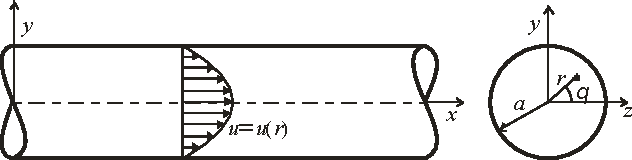
\includegraphics{ej7}
\end{center}

Suponiendo despreciables las fuerzas de cuerpo, hallar la solución de la forma

\begin{align*}
u &= u(r) & v &= 0 & w &= 0
\end{align*}

Use la siguiente relación entre el \textit{Laplaciano} de una función $f$ en coordenadas cartesianas $(x,y,z)$ y en coordenadas cilíndricas $(x,r,\theta)$:

\begin{align*}
\nabla^{2}f &= \frac{\partial^{2}f}{\partial x^{2}}
+\frac{\partial^{2}f}{\partial y^{2}}+\frac{\partial^{2}f}{\partial z^{2}}
=\frac{\partial^{2}f}{\partial x^{2}}
+\frac{1}{r}\frac{\partial}{\partial r}\left(r\frac{\partial f}{\partial r}\right)
+\frac{1}{r^{2}}\frac{\partial^{2}f}{\partial\theta^{2}}
\end{align*}

\begin{quote}
\begin{tcolorbox}[colback=gray!10!white,colframe=black!0!white]

\begin{align*}
\frac{Du}{Dt} &= \frac{\partial u}{\partial t}+\mathbf{\nu}\cdot\nabla u
& \frac{\partial p}{\partial x} &= -G \\
\frac{Du}{Dt} &= X-\frac{1}{\rho}\frac{\partial p}{\partial x}+\nu\nabla^{2}u \\
\frac{1}{\rho}G+\nu\nabla^{2}u &= 0 
& \nu &= \frac{u}{\rho} \\
\frac{1}{\rho}G+\frac{u}{\rho}\left(\frac{\partial^{2}u}{\partial x^{2}}
+\frac{\partial^{2}u}{\partial y^{2}}+\frac{\partial^{2}u}{\partial z^{2}}\right) &= 0 \\
G+u\left(\frac{\partial^{2}u}{\partial x^{2}}+\frac{\partial^{2}u}{\partial y^{2}}
+\frac{\partial^{2}u}{\partial z^{2}}\right) &= 0 \\ \\
\frac{\partial^{2}u}{\partial y^{2}}+\frac{\partial^{2}u}{\partial z^{2}} &= -\frac{G}{\mu} \\
\frac{1}{r}\frac{\partial}{\partial r}\left(r\frac{\partial u}{\partial r}\right)
&= -\frac{G}{\mu} \\
r\frac{\partial u}{\partial r} &= -\int\frac{G}{\mu}r\,dr=-\frac{G^{2}}{2\mu}+A \\
\frac{\partial u}{\partial r} &= -\frac{G}{2\mu}r+\frac{A}{r} \\
u(r) &= -\frac{G}{4\mu}r^{2}+A\ln{r}+B
\end{align*}

Sea $A=0$ entonces salvamos el problema del logaritmo cuando $r=0$.

\begin{align*}
u(r) &= -\frac{G}{4\mu}r^{2}+B \\
u(r=a) &= 0 \\
u(a) &= -\frac{Ga^{2}}{4\mu}+B=0 & B &= \frac{Ga^{2}}{4\mu}
& u(r) &= \frac{G}{4\mu}(a^{2}-R^{2})
\end{align*}

\end{tcolorbox}
\end{quote}

Con la solución hallada, mostrar que:

\begin{enumerate}[a.]
\item La tasa de flujo de masa a través del tubo es $\displaystyle Q=-\frac{\pi a^{4}\rho}{8}\nabla^{2}u$

\begin{quote}
\begin{tcolorbox}[colback=gray!10!white,colframe=black!0!white]

\begin{align*}
Q &= \int_{S}\rho v_{j}\nu_{j}dS \\
&= \int_{S}\rho\mu dS \\
&= \int_{0}^{a}\rho\mu 2\pi r\,dr \\
&= \int_{0}^{a}\frac{\rho G}{4\mu}(a^{2}-r^{2})2\pi r\,dr \\
&= \int_{0}^{a}\frac{6\pi\rho}{2\mu}\left(a^{2}r-r^{3}\right)dr \\
&= \frac{6\pi\rho}{2\mu}\left(\left.\frac{a^{2}r^{2}}{2}\right|_{0}^{a}
-\left.\frac{r^{4}}{4}\right|_{0}^{a}\right) \\
&= \frac{6\pi\rho}{2\mu}\left(\frac{a^{4}}{2}-\frac{a^{4}}{4}\right) \\
&= \frac{6\pi\rho}{8\mu}a^{4} \\
&= -\frac{\rho\pi a^{4}\nabla^{2}u}{8}
\end{align*}

\end{tcolorbox}
\end{quote}

\item La velocidad media es $\displaystyle u_{m}=-\frac{a^{2}}{8}\nabla^{2}u$

\begin{quote}
\begin{tcolorbox}[colback=gray!10!white,colframe=black!0!white]

\begin{align*}
u_{m} &= \frac{1}{|\Omega|}\int_{\Omega}u\,d\Omega \\
&= \frac{1}{\pi a^{2}}\int_{0}^{a}\frac{G}{4\mu}(a^{2}-r^{2})2\pi r\,dr \\
&= \frac{G}{2a^{2}\mu}\left(\left.\frac{a^{2}r^{2}}{2}\right|_{0}^{a}
-\left.\frac{r^{4}}{4}\right|_{0}^{a}\right) \\
&= \frac{Ga^{2}}{8\mu} \\
&= -\frac{a^{2}}{8}\nabla^{2}u
\end{align*}

\end{tcolorbox}
\end{quote}

\item El coeficiente de fricción en la pared es

\begin{align*}
c_{f} &= \frac{\textit{Tensión cortante}}{\textit{Presión dinámica media}}
=\frac{-\mu\frac{\partial u}{\partial r}\left|_{r=a}\right.}{\frac{1}{2}\rho u_{m}^{2}}=\frac{16}{R_{N}}
\end{align*}

donde $\displaystyle R_{N}=\frac{2a\rho u_{m}}{\mu}$ es un número de \textit{Raynolds}.

\begin{quote}
\begin{tcolorbox}[colback=gray!10!white,colframe=black!0!white]

\begin{align*}
\frac{\partial u}{\partial r} &= \left.-\frac{G}{2\mu}r\right|_{r=a} \\
&= -\frac{G}{2\mu}a \\
&= \frac{\frac{Ga}{2}}{\frac{1}{2}\rho\frac{a^{2}}{8}\frac{G}{\mu}u_{m}} \\
&= \frac{\frac{Ga}{2}}{\frac{\rho}{16}a^{2}\frac{G}{\mu}u_{m}} \\
&= \frac{16Ga\mu}{2\rho a^{2}G u_{m}} \\
&= \frac{16\mu}{2\rho a u_{m}} \\
&= \frac{16}{R_{N}}
\end{align*}

\end{tcolorbox}
\end{quote}

\end{enumerate}

\section*{Apéndice}

\textit{Teorema de Gauss (transforma integrales de superficie en integrales de volumen):}

\begin{equation}
\int_{V}\frac{\partial A}{\partial x_{i}}dV=\int_{S}A\nu_{i}dS
\label{eq:tg}
\end{equation}

\vspace{1em}

\textit{Derivada material:}

\begin{equation}
\frac{DA}{Dt}=\frac{\partial A}{\partial t}+\mathbf{\nu}\cdot\nabla A
=\frac{\partial A}{\partial t}+\nu_{i}\cdot\frac{\partial A}{\partial x_{i}}
=\frac{\partial A}{\partial t}+\left(
\nu_{1}\frac{\partial A}{\partial x_{1}}
+\nu_{2}\frac{\partial A}{\partial x_{2}}
+\nu_{3}\frac{\partial A}{\partial x_{3}}
\right)
\label{eq:dm}
\end{equation}

\vspace{1em}

\textit{Raynolds:}

\begin{align}
\frac{D}{Dt}\int_{V}A\,dV
&= \int_{V}\frac{\partial A}{\partial t}dV
+\int_{V}\frac{\partial}{\partial x_{j}}(A\nu_{j})dV \\
&= \int_{V}\left(\frac{DA}{Dt}+A\frac{\partial\nu_{j}}{\partial x_{j}}\right)dV
\end{align}

\vspace{1em}

\textit{Ecuaciones de continuidad:}

\begin{align}
\frac{D\rho}{Dt}+\rho\frac{\partial\nu_{j}}{\partial x_{j}} &= 0
& \textit{Si el fluido es incompresible la densidad es constante.}
&& \frac{D\rho}{Dt} &= 0 \\
\rho\frac{\partial\nu_{j}}{\partial x_{j}} &= 0
\end{align}

\vspace{1em}

\textit{Ecuación de movimiento:}

\begin{equation}
\rho\frac{D\nu_{i}}{Dt}=\frac{\partial\sigma_{ij}}{\partial x_{j}}+X_{i}
\label{eq:em}
\end{equation}


\begin{thebibliography}{99}
\bibitem{MCF}
Y. C. Fung,
\emph{A First Course in Continuum Mechanics}, 
tercera edición,
PRENTICE HALL,
1994.
\end{thebibliography}

\end{document}